\documentclass[a4paper]{article}

\usepackage{hyperref}
\usepackage{amsmath}
\usepackage{mathtools}
\usepackage[german]{babel}
\usepackage[utf8]{inputenc}
\usepackage{amsfonts}
\usepackage{graphicx}
\usepackage{siunitx}
\usepackage{tabularx}
\usepackage{wrapfig}
\usepackage{float}
\usepackage[margin=2cm]{geometry}


%opening
\title{}
\author{}
\title{Abiturvorbereitung Physik}
\author{Noah Peeters\\ Schüler, Otto-Hahn-Gymnasium Geesthacht, Germany}

\begin{document}
	
	\pagenumbering{gobble}
	\maketitle
	\newpage
	\pagenumbering{arabic}
	
	\tableofcontents
	\listoffigures
	\listoftables
	\newpage
	
	\section{Kinematik}
		\subsection{Charakteristische Größen}
			\begin{table}[H]
				\def\arraystretch{1.5}
				\begin{tabularx}{\textwidth}{|c|c|c|X|}\hline
					Größe & Einheit & Formel & Beschreibung \\\hline
					$s(t)$ & \si{\meter} & $s(t) = \frac{a}{2}\cdot t^2+v_0\cdot t+s_0$ & Die Position beschreibt, wie weit sich ein Objekt bewegt hat.\\\hline
					$v(t)$ & \si{\meter\per\second}  & $v(t) = \dot{s}(t) = a\cdot t+v_0$ & Die Geschwindigkeit beschreibt, wie schnell sich ein Objekt relativ zu einem Bezugspunkt bewegt.\\\hline
					$a(t)$ & \si{\meter\per\second\squared} & $a(t) = \dot{v}(t) = \ddot{s}(t) = a$ & Die Beschleunigung beschreibt, wie sich die Geschwindigkeit eines Objektes verändert.\\\hline
				\end{tabularx}
				\caption {Charakteristische Größen der Kinematik}
				\label{table:kinematik_grossen}
			\end{table}
		
		\subsection{Wichtige Bewegungen}
			\subsubsection{Freier Fall}
				Der freie Fall ist eine idealisierte Bewegung ohne Energieverlust oder Reibung. Auf das Objekt wirkt im freien Fall nur die Gravitationskraft einer einzigen punktförmigen Masse. Das Objekt startet bei der Höhe $h_0$ ohne eine Geschwindigkeit. Die Beschleunigung $a$ ist immer senkrecht nach unten gerichtet. Auf der Erde gilt nährungsweise $a=g\approx9.81$. Damit ergibt sich das Bewegungsgesätz
				
				\begin{equation}
					h(t) = h_0 - \frac{a}{2}\cdot t^2
				\end{equation}
			
			\subsubsection{Waagerechter Wurf}
				Der waagerechte Wurf ist wieder eine idealisierte Bewegung ohne Energieverlust oder Reibung. Auf das Objekt wirkt während des Fluges nur die Gravitationskraft einer einzigen punktförmigen Masse. Beim waagerechten Wurf startet das Objekt ebenfalls bei der Höhe $h_0$ und die Beschleunigung $a$ ist ebenfalls senkrecht nach unten gerichtet. Das Objekt startet jedoch mit einer zur Beschleunigung \textit{senkrecht} stehenden Geschwindigkeit $v_{x,0}$. Der waagerechte Wurf lässt sich als \textit{Überlagerung} zweier Bewegungen, eine in x-Richtung und eine in y-Richtung, beschreiben:
				
				\begin{equation}\label{waagerechter_wurf:h}
					h(t) = h_0 - \frac{a}{2}\cdot t^2
				\end{equation}
				
				\begin{equation}\label{waagerechter_wurf:x}
					x(t) = v_{x,0}\cdot t
				\end{equation}
				Mithilfe von Gleichung \ref{waagerechter_wurf:h} kann man nun die Zeit berechnen, die das Obejekt braucht, um den Wurf zu beenden. Daf\"ur wird $h_0$ mit $0$ gleichgesetz (unter der Annahme, dass sich auf Höhe $0$ der Boden befindet):
				
				\begin{equation}
					h(t) = 0 =  h_0 - \frac{a}{2}\cdot t^2
				\end{equation}
				\begin{equation}\label{waagerechter_wurf:t}
					t = \sqrt{\frac{2h_0}{a}}
				\end{equation}
				Setzt man nun Gleichung \ref{waagerechter_wurf:t} in Gleichung \ref{waagerechter_wurf:x}  ein, erhält man die Strecke, die während des Fluges in x-Richtung zer\"uckgelegt wurde:
			
				\begin{equation}
					x(t) = v_{x,0}\cdot\sqrt{\frac{2h_0}{a}}
				\end{equation}
				
			\subsubsection{Schräger Wurf}
				Der schräge Wurf ist eine besonder Form des waagerechten Wurfs, bei dem die Geschwindigkeit nicht senkrecht zur Beschläunigung steht. Der winkel zwischen der initiale Geschwindigkeit $v_0$ und der zur Beschläunigung senkrecht stehenden Ebene wird mit $\alpha$ bezeichnet. Nun kann man die initiale Geschwindigkeit wie folgt in ihre x und y Komponente aufgeteilt werden:
				
				\begin{equation}
					v_{x,0} = \cos(\alpha)\cdot v_0
				\end{equation}
				\begin{equation}
					v_{y,0} = \sin(\alpha)\cdot v_0
				\end{equation}
				Mit diesen beiden Geschwindigkeiten kann man wieder den Wurf als zwei \"uberlagerte Bewegungen betrachten:
				
				\begin{equation}
					h(t) = h_0 - \frac{a}{2}\cdot t^2 - v_{y,0}\cdot t = h_0 - \frac{a}{2}\cdot t^2 - \sin(\alpha)\cdot v_0\cdot t
				\end{equation}
				
				\begin{equation}
					x(t) = v_{x,0}\cdot t = \cos(\alpha)\cdot v_0\cdot t
				\end{equation}
			
	\section{Dynamik}
		\subsection{Charakteristische Größen}
	
			\begin{table}[H]
				\def\arraystretch{1.5}
				\begin{tabularx}{\textwidth}{|c|c|c|X|}\hline
					Größe & Einheit & Formel & Beschreibung \\\hline
					$\vec{p}$ & \si{\kg\meter\per\second} & $\vec{p} = m\cdot \vec{v}$ & Der Impuls.\\\hline
					$\vec{F}$ & \si{\newton}=\si{\kg\meter\per\second\squared}  & $	\vec{F} = m\cdot \vec{a}$ & Die Kraft.\\\hline
					$E$ & \si{\joule}=\si{\kg\meter\squared\per\second\squared} &\hyperref[energie_kin]{$E_{kin}$}; \hyperref[energie_pot]{$E_{Pot}$}  & Die Energie.\\\hline
				\end{tabularx}
				\caption {Charakteristische Größen der Dynamik}
				\label{table:dynamik_grossen}
			\end{table}
	
			\subsubsection{Impuls}
			
				Der Impuls lässt sich umgangssprachlich als ''Schwung'' oder ''Wucht'' beschreiben. Er ist eine vektorielle Größe und sowohl zur Masse als auch zur Geschwindigkeit eines Körpers proportional:
				
				\begin{equation}
					\vec{p} = m\cdot \vec{v}
				\end{equation}
				Da $m$ eine skalare Größe ist, sind $\vec{p}$ und $\vec{v}$ gleich ausgerichtet. Die Summe alle Impulse in einem abgeschlossenen System bleibt konstant. Es gilt der Impulserhaltungssatz: $\vec{p_1} + \vec{p_2} + ... + \vec{p_n} = \vec{p} = const$.
			
			\subsubsection{Kräfte}
			
				Die Kraft ist eine vektorielle Größe und zur Masse sowie zur Beschleunigung des Körpers proportional:
				
				\begin{equation}\label{kraft:fma}
					\vec{F} = m\cdot \vec{a}
				\end{equation}
				Da $m$ eine skalare Größe ist, sind $\vec{F}$ und $\vec{a}$ gleich ausgerichtet. Es gelten die Newton'schen Gesetze:
				
				\begin{enumerate}
					\item Wenn die Summe aller auf einen Körper wirkenden Kräfte null ist, bleibt die Geschwindigkeit konstant: $\vec{v} = const$ wenn $\vec{F} = 0$.
					\item Es gilt $\vec{F} = m\cdot \vec{a}$.
					\item Zu jeder wirkende Kraft wirkt eine ihr vom Betrag her gleich große Kraft in die entgegengesetzte Richtung: $\vec{F_1} = -\vec{F_2}$ \textit{(Actio gleich Reactio)}.
				\end{enumerate}
		
			\subsubsection{Energien in der klassischen Mechanik}
			
				Die Energie in einem abgeschlossenen System bleibt konstant. Es gilt der Energieerhaltungssatz: $\vec{E_1} + \vec{E_2} + ... + \vec{E_n} = \vec{E} = const$.\\
				Die Energie lässt sich in verschiedene Formen einteilen.
				
				\paragraph{Kinetische Energie (Bewegungsenergie)}\label{energie_kin}
					Die kinetische Energie beschreibt die Energie, die in Form von Bewegung gespeichert ist. Sie lässt sich folgendermaßen berechnen:
					
					\begin{equation}\label{energie_kin_eq}
						E_{kin} = \frac{1}{2}\cdot m\cdot v^2
					\end{equation}
					
				\paragraph{Potenzielle Energie (Lageenergie)}\label{energie_pot}
					Die potenzielle Energie beschreibt die Energie, die in der Lage oder Position einer Masse gespeichert ist. Die potenzielle Energie einer sich in eiem Gravitationsfeld befindenden Masse mit der Beschleunigung $a$ lässt sich folgendermaßen berechnen:
					
					\begin{equation}
						E_{pot} = m\cdot a \cdot s
					\end{equation}
					Zusammen mit der Gleichung \ref{kraft:fma} erhält man:
					
					\begin{equation}\label{energie:fs}
						E_{pot} = \vec{F} \cdot s
					\end{equation}
	
		\subsection{Anwendungen}
			\subsubsection{Newtonpendel}
				Beim Newtonpendel hängen mehrere gleich schwere Kugeln mit jeweils der Masse $m$ in einer Reihe an Fäden. Hebt man nun $n_1 \in \mathbb{N}$ Kugeln seitlich hoch und lässt sie dann schwingen, sodass es einen zentralen Stoß mit den restlichen Kugeln gibt, bei der die schwingenden Kugeln die Geschwindigkeit $v$ haben, entfernen sich an der anderen Kugelreihenseite $n_2 \in \mathbb{N}$ Kugeln mit der Geschwindigkeit $u$. Um zu beweisen, dass $n_1 = n_2$ ist, muss man sowohl den Impuls- als auch den Energieerhalungssatz anwenden, aus dem sich jedoch jeweils die Masse rauskürzen lässt:
				
				\begin{equation}
					p=n_1\cdot m \cdot v = n_2\cdot m \cdot u
				\end{equation}
				\begin{equation}\label{newtonpendel:p_short}
					n_1\cdot v = n_2 \cdot u
				\end{equation}
				\begin{equation}
					E=\frac{1}{2}\cdot n_1\cdot m \cdot v^2 = \frac{1}{2}\cdot n_2\cdot m \cdot u^2
				\end{equation}
				\begin{equation}\label{newtonpendel:e_short}
					n_1 \cdot v^2 = n_2 \cdot u^2
				\end{equation}
				Nun kann man Gleichung \ref{newtonpendel:p_short} zu $u$ umstellen, und diese anschließend in die Gleichung \ref{newtonpendel:e_short} einsetzen.
			
				\begin{equation}
					u = \frac{n_1\cdot v}{n_2}
				\end{equation}
				
				\begin{equation}
					n_1 \cdot v^2 =n_2 \cdot \left(\frac{n_1\cdot v}{n_2}\right) ^2\Leftrightarrow n_1 = n_2
				\end{equation}

	
			\subsubsection{Elastischer Stoß}
			
				Treffen zwei Körper mit den Massen $m_1$ und $m_2$ und den Geschwindigkeiten $v_1$ und $v_2$ elastisch aufeinander, kommt es zum elastischen Stoß. Wenn die Geschwindigkeiten nach dem Stoß mit $u_1$ und $u_2$ bezeichnet werden, gilt nach dem Impuls- und Energieerhalungssatz:\\\\
				Impulserhaltung:
				\begin{equation}
					p=m_1 \cdot v_1 + m_2 \cdot v_2 = m_1 \cdot u_1 + m_2 \cdot u_2
				\end{equation}
				\begin{equation}\label{elastischer_stoss:p_short}
					m_1 \cdot (v_1 - u_1) = m_2 \cdot (u_2 - v_2)
				\end{equation}
				Energieerhaltung:
				\begin{equation}
					E=\frac{1}{2}m_1 \cdot v_1 + \frac{1}{2}m_2 \cdot v_2 = \frac{1}{2}m_1 \cdot u_1 + \frac{1}{2}m_2 \cdot u_2
				\end{equation}
				\begin{equation}
					m_1 \cdot (v_1^2 - u_1^2) = m_2 \cdot (u_2^2 - v_2^2)
				\end{equation}
				\begin{equation}\label{elastischer_stoss:e_short}
					m_1 \cdot (v_1 - u_1)(v_1 + u_1)= m_2 \cdot (u_2 - v_2)(u_2 + v_2)
				\end{equation}
				Nun kann man Gleichung \ref{elastischer_stoss:p_short} in Gleichung \ref{elastischer_stoss:e_short} einsetzen:
				\begin{equation}
					m_2 \cdot (u_2 - v_2)(v_1 + u_1)= m_2 \cdot (u_2 - v_2)(u_2 + v_2)
				\end{equation}
				\begin{equation}\label{elastischer_stoss:u1_u2}
					v_1 + u_1= u_2 + v_2
				\end{equation}
				Setzt man Gleichung \ref{elastischer_stoss:u1_u2} zu $u_2$ oder $u_1$ umgestellt in Gleichung \ref{elastischer_stoss:p_short} ein, erhält man Formeln für $u_1$ und $u_2$:
				
				\begin{equation}
					u_1=\frac{m_2(2v_2 - v_1) + m_1v_1}{m_1+m_2}
				\end{equation}
				\begin{equation}
					u_2=\frac{m_1(2v_1 - v_2) + m_2v_2}{m_1+m_2}
				\end{equation}
	
			\subsubsection{Unelastischer Stoß}
			
				Treffen zwei Körper mit den Massen $m_1$ und $m_2$ und den Geschwindigkeiten $v_1$ und $v_2$ unelastisch aufeinander, kommt es zum unelastischen Stoß. Das heißt, die Körper lösen sich nach dem Stoß nicht voneinander. Wenn die Geschwindigkeit des neuen Körpers nach dem Stoß mit $u$ bezeichnet wird, gilt nach dem Impuls- und Energieerhalungssatz:
				
				\begin{equation}\label{unelastischer_stoss:p}
					p=m_1 \cdot v_1 + m_2 \cdot v_2 = (m_1 + m_2) \cdot u
				\end{equation}
				Für die Geschwindigkeit $u$ ergibt sich nach Gleichung \ref{unelastischer_stoss:p}:
				
				\begin{equation}
					u=\frac{m_1 \cdot v_1 + m_2 \cdot v_2}{m_1 + m_2}
				\end{equation}
			
			
	\section{Schwingungen und Wellen}			
		\subsection{Charakteristische Größen}

	
			\begin{table}[H]
				\def\arraystretch{1.5}
				 \begin{tabularx}{\textwidth}{|c|c|c|X|}\hline
					Größe & Einheit & Formel & Beschreibung \\\hline
					$T$ & \si{\second} & & Die Zeit für eine vollständige Periode.\\\hline
					$f$ & \si{\hertz}  & & Das Reziprok der Zeit für eine vollständige Periode.\\\hline
					$\lambda$ & \si{\hertz} & & Die räumliche Ausdehnung einer Periode.\\\hline
					$\hat{y}$ & \si{\meter}& & Die Amplitude der Schwingung beschreibt die maximale Auslenkung.\\\hline
					$\omega$ & \si{\hertz} & $\omega=\frac{2\pi}{T}$ & Die Winkelgeschwindigkeit des Zeigers im Zeigermodell.\\\hline
					$y(t, x)$ & \si{\meter} & $\hat{y}\cdot\sin\left(2\pi\left(\frac{t}{T}-\frac{x}{\lambda} \right)\right)$ & Die Elongation beschreibt die Auslenkung zu einem bestimmten Zeitpunkt $t$ an einem bestimmten Ort $x$.\\\hline
					$v(t, x)$ & \si{\meter} & $\hat{y}\cdot\omega\cdot\cos\left(2\pi\left(\frac{t}{T}-\frac{x}{\lambda} \right)\right)$ & Die Geschwindigkeit beschreibt die Schwinggeschwindigkeit zu einem bestimmten Zeitpunkt $t$ an einem bestimmten Ort $x$.\\\hline
					$a(t, x)$ & \si{\meter} & $-\hat{y}\cdot\omega^2\cdot\sin\left(2\pi\left(\frac{t}{T}-\frac{x}{\lambda} \right)\right)$ & Die Beschleunigung beschreibt die Schwingbeschleunigungzu einem bestimmten Zeitpunkt $t$ an einem bestimmten Ort $x$.\\\hline
					$c$ & \si{\meter\per\second} & $c=\lambda\cdot f = \frac{\lambda}{T}$ & Die Geschwindigkeit der räumlichen Ausbreitung.\\\hline
				\end{tabularx}
				\caption {Charakteristische Größen für Schwingungen und Wellen}
				\label{table:wellen_grossen}
			\end{table}	
	
		\subsection{Herleitung von $y(t, x)$}
			Zum Zeitpunkt $t$ hat die Welle $\frac{t}{T}$ von einer vollen Phase also von $2\pi = 360\si{\degree}$ geschafft. Damit ist die Phase $\varphi = 2\pi\cdot\frac{t}{T} = \frac{2\pi}{T}\cdot t$. Die Elongation lässt sich mithilfe eines rechtwinkligen Dreiecks wie es in Abbildung \ref{img:welle_zeigerdarstellung} als $y=\hat{y}\cdot sin\left(\varphi\right)$ bestimmen. Damit gilt
			
			\begin{equation}\label{einfache_wellengleichung}
				y=\hat{y}\cdot sin\left(\frac{2\pi}{T}\cdot t\right)
			\end{equation}
			
			
			\begin{figure}[h]
				\centering
				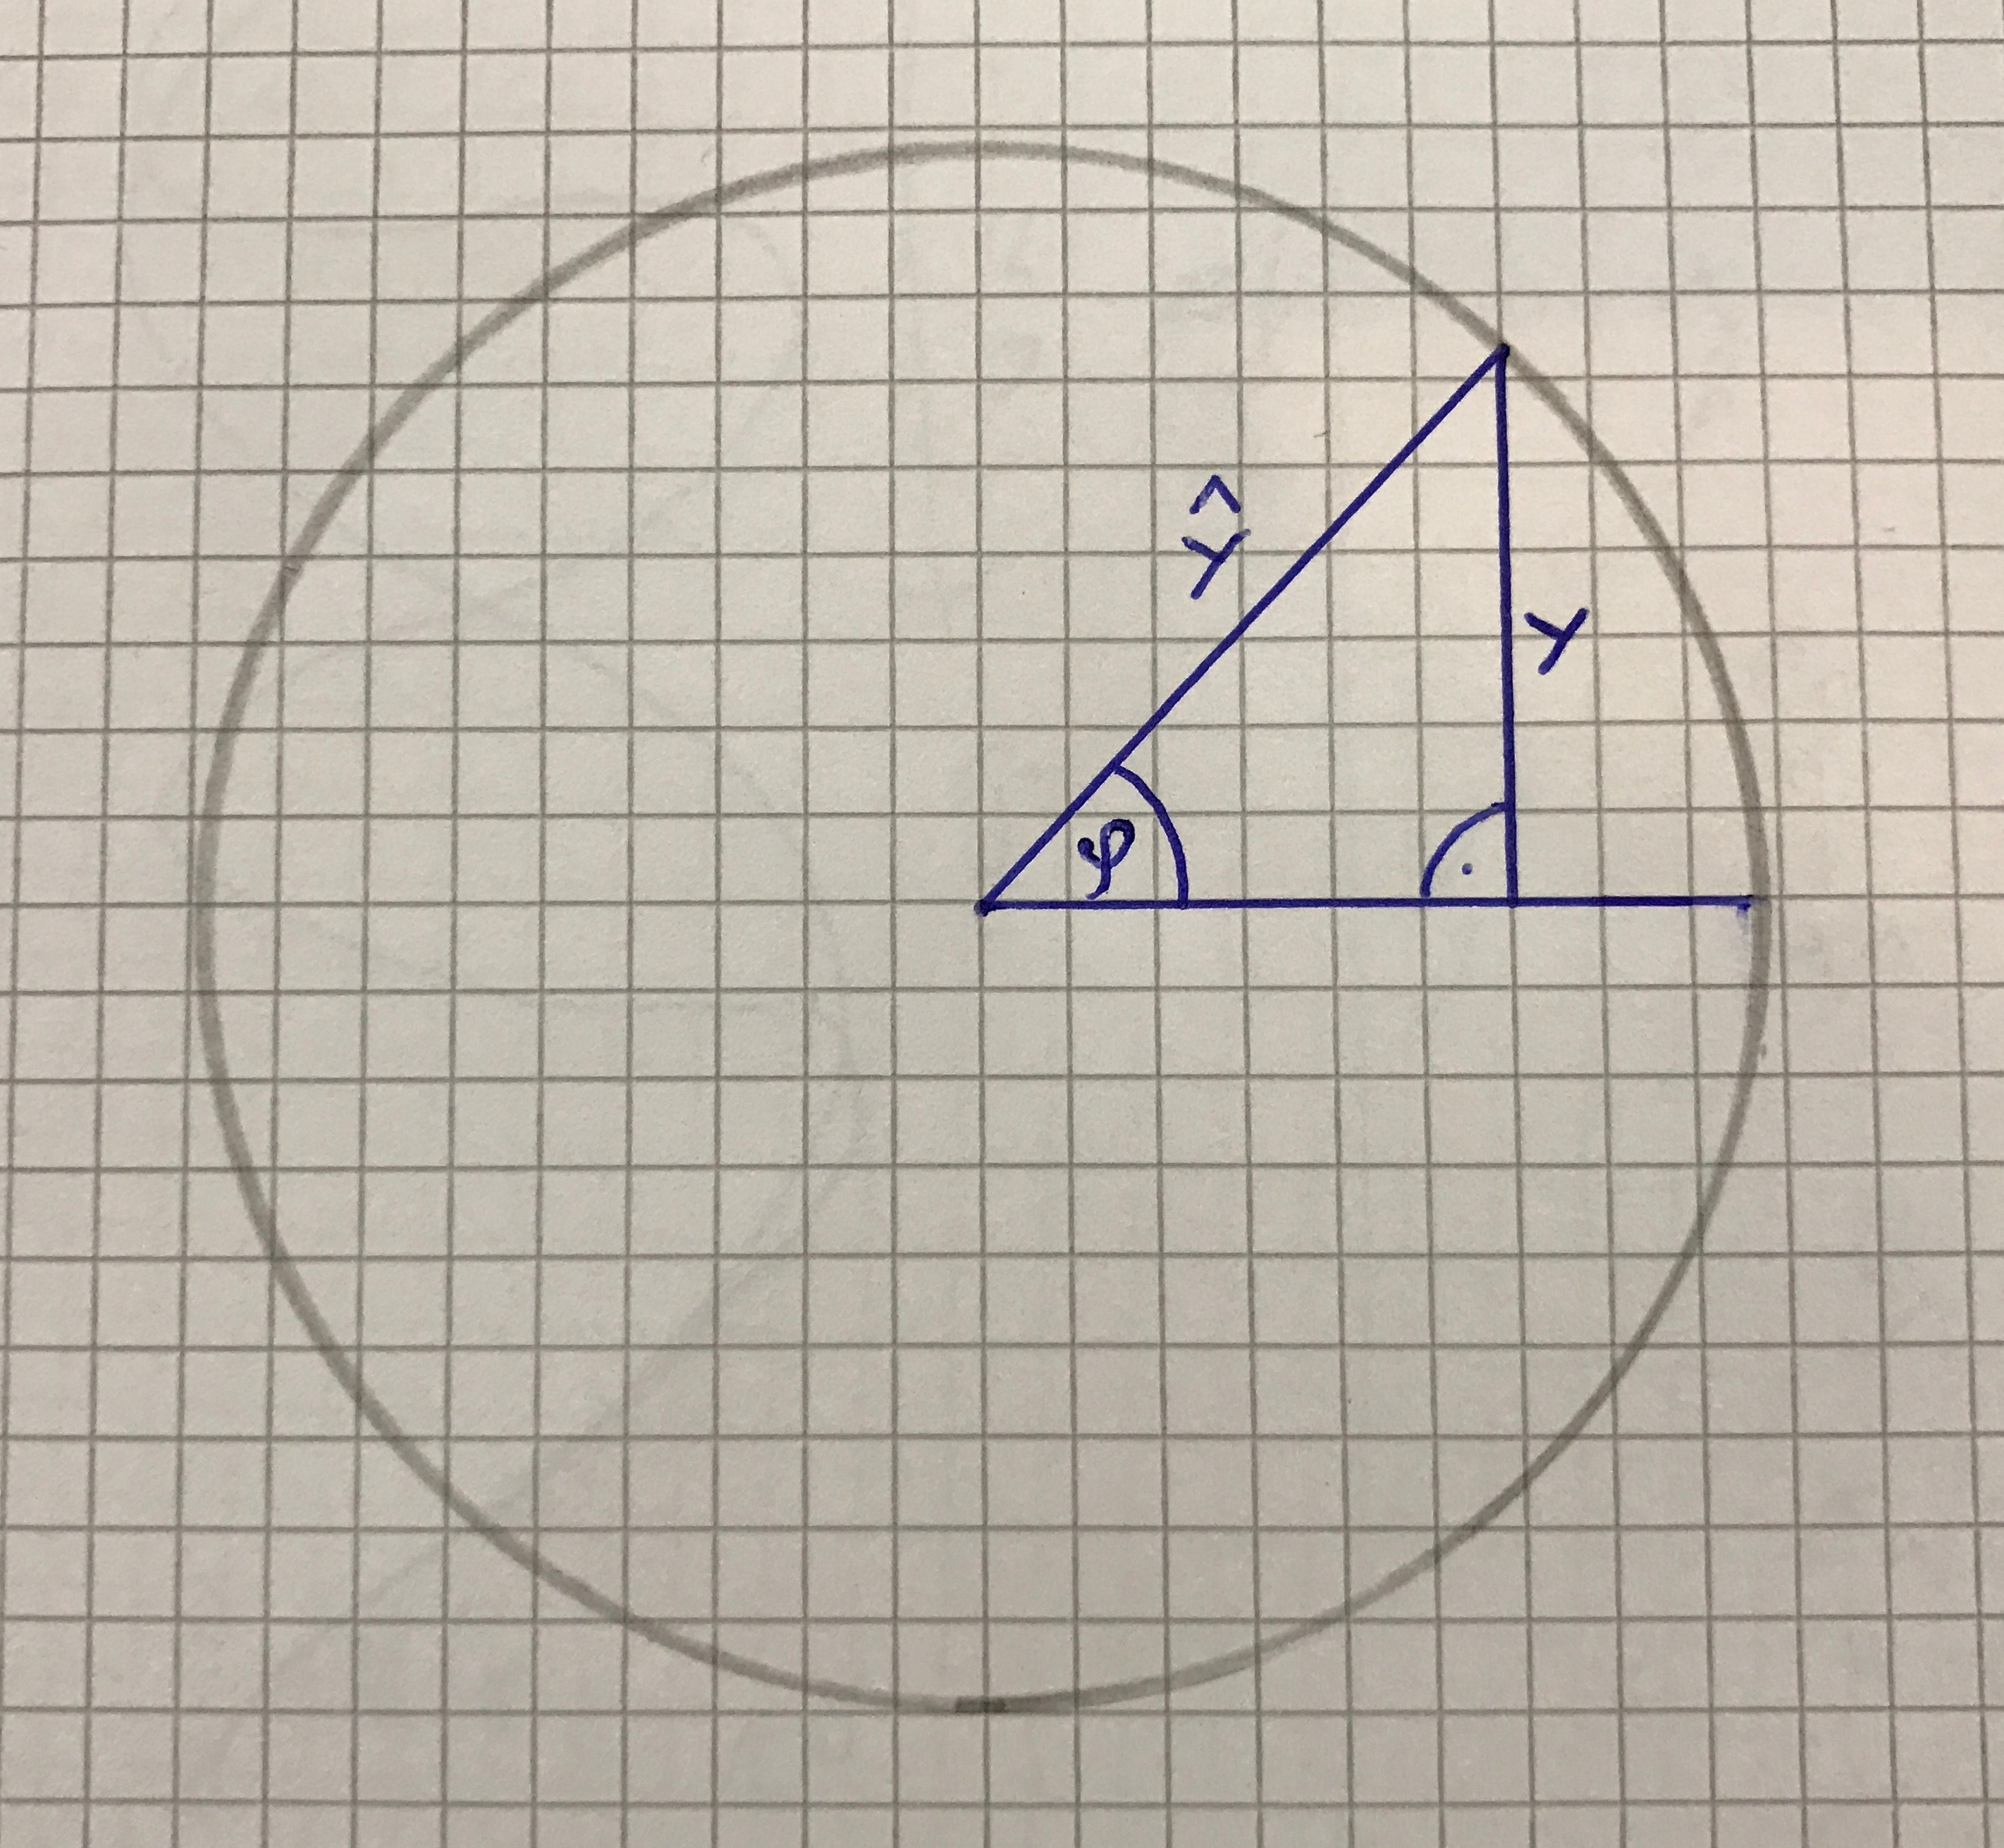
\includegraphics[width=0.48\textwidth]{img/welle_zeigerdarstellung.jpg}
				\caption{Die Elongation bei dem Phasenwinkel $\varphi$}
				\label{img:welle_zeigerdarstellung}
			\end{figure}
		
		
			\noindent Betrachtet man nun nicht den Ort $x_0 = 0$ sondern $x_0=x$, setzt die Welle erst später ein, da die Strecke $x$ erst zurückgelegt werden muss. Genauso gut kann man sagen, dass $\varphi_0=0$ gilt, wenn die Welle den Ort $x_0=x$ erreicht. Die Wellengleichung \ref{einfache_wellengleichung} um $\varphi_0$ erweitert lautet
		
			\begin{equation}\label{wellengleichung_phi0}
				y=\hat{y}\cdot sin\left(\frac{2\pi}{T}\cdot t + \varphi_0\right)
			\end{equation}			
			
			

		\subsection{Harmonischer Oszillator}
			\begin{figure}[H]
				\centering
				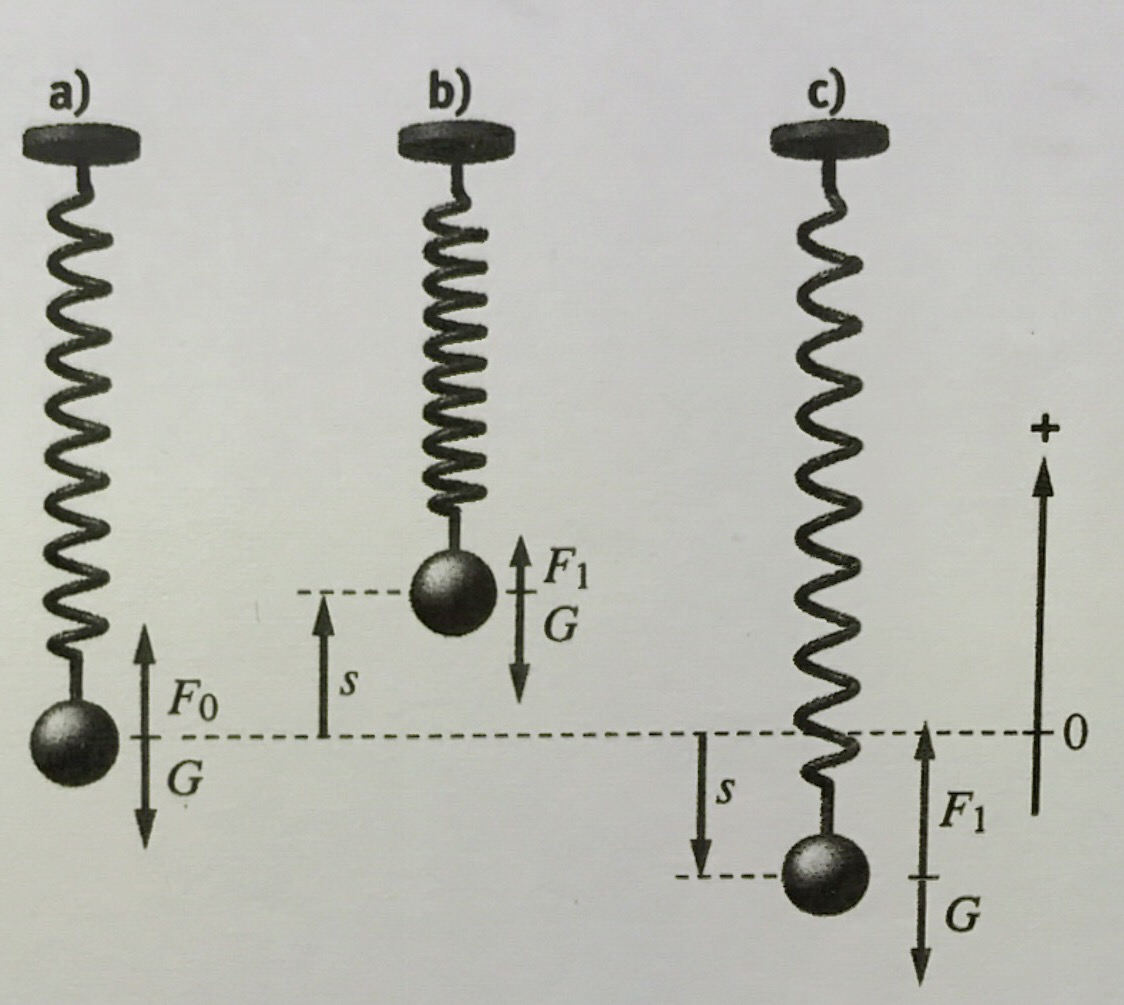
\includegraphics[width=0.48\textwidth]{img/Federpendel_001.jpg}
				\caption{Das Federpendel mit der Auslenkung $s$}
				\label{img:federpendel_001}
			\end{figure}
		

	
			In der in Abbildung \ref{img:federpendel_001}a dargestellten Gleichgewichtslage ist die nach oben gerichtete und damit positive Federkraft $F_0$ vom Betrag her genau so groß wie die nach unten gerichtete und damit negative Gewichtskraft $G$. Es gilt $G=-F_0$ und damit
			\begin{equation}
				F=G+F_0=0
			\end{equation}
			Wenn man den Körper wie in Abbildung \ref{img:federpendel_001}b zu sehen um die Strecke $s$ nach oben auslängt, wird $F_1$ kleiner: $F_1 = F_0-Ds$. Mit der Nährung, dass $G$ konstant bleibt, gilt:
			\begin{equation}
				F=G+F_0-Ds = G+F_1= -Ds
			\end{equation}
			Analog wird $F_1$ bei einer Auslänkung nach unten größer: $F_1 = F_0-Ds$. Da $s$ in Abbildung \ref{img:federpendel_001}c kleiner $0$ ist, ist $-Ds$ positiv. Damit ist auch in Fall c die resultierende Kraft
			\begin{equation}\label{harmonischer_oszillator:fds}
				F=G+F_0-Ds = G+F_1= -Ds
			\end{equation}
			Die Rückstellkraft $F$ ist also proportional zur Elongation $s$. Das negative Vorzeichen, beschreibt, dass die Kraft immer entgegen der Elongationsrichtung steht. Sie wirkt also immer zur Gleichgewichtslage.
			\begin{equation}
				F= -Ds
			\end{equation}
			Mithilfe der Beschleunigungsgleichung $a(t)=-\hat{y}\cdot\omega^2\cdot\sin\left(\omega\cdot t\right)$ und Newtons Gleichung für die Kraft (Gleichung \ref{kraft:fma}) erhalten wir:
			\begin{equation}\label{harmonischer_oszillator:fma}
				F= m\cdot a = -m\cdot \hat{y}\cdot\omega^2\cdot\sin\left(\omega\cdot t\right)
			\end{equation}
			Da $s=\hat{s} \cdot\sin(\omega\cdot t)$ gilt, können wir die Gleichung \ref{harmonischer_oszillator:fma} wie folgt vereinfachen:
			\begin{equation}
				F= m\cdot a = -m\cdot\omega^2\cdot s
			\end{equation}
			Diese können wir mit Gleichung \ref{harmonischer_oszillator:fds} gleichsetzen und erhalten:
			\begin{equation}
				-m\cdot\omega^2\cdot s = -Ds \Leftrightarrow D=m\cdot\omega^2
			\end{equation}
			Setzten wir nun $\omega=\frac{2\pi}{T}$ ein, erhalten wir eine Formel für die Periodendauer T:
			\begin{equation}
				T=2\pi\cdot\sqrt{\frac{m}{D}}
			\end{equation}
	
		\subsection{Doppelspalt}
	
		\subsection{Überlagerung von harmonsichen Schwingungen}
	
			\subsubsection{Überlagerung gleicher Frequenzen}
			
				Überlagert man zwei Schwingungen mit gleicher Frequenz erhällt man wieder eine harmonische Schwingung mit derselben Frequenz. Phase und Amplitude egeben sich aus vektorieller Addition.
			
			\subsubsection{Überlagerung unterschiedlicher Frequenzen und Schwebung}
			
				Überlagert man zwei Schwingungen mit unerschiedlichen Frequenzen $f_1$ und $f_2$ überlagern sie sich zu einer Schwebung. Es entsteht deshalb auch \textit{keine} harmonische Schwingung. Die neue Schwingung hat die Grundfrequenz
				
				\begin{equation}
					f=\frac{f_1+f_2}{2}
				\end{equation}
				die Schwebungsfrequenz
				
				\begin{equation}
					f_s=|f_1-f_2|
				\end{equation}
				und die Modulationsfrequenz
				
				\begin{equation}
				f_{mod}=\frac{|f_1-f_2|}{2}
				\end{equation}
				
				\begin{figure}[H]
					\centering
					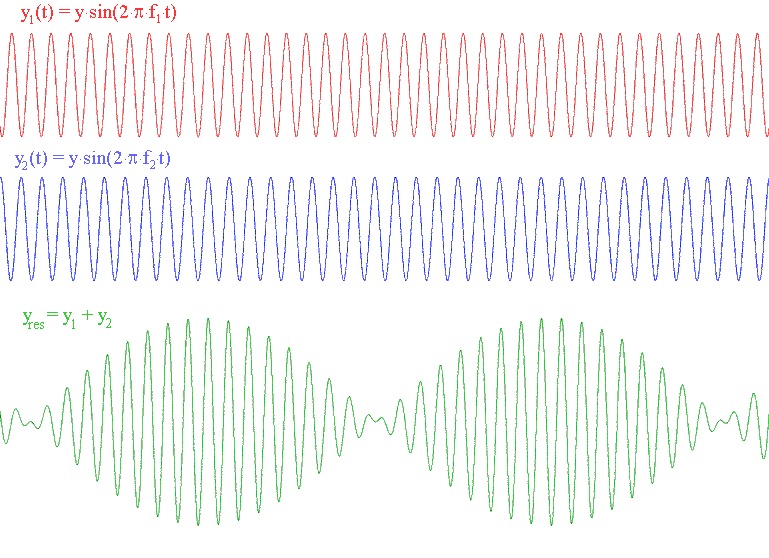
\includegraphics[width=0.5\textwidth]{img/schwebung_k_akustwellen_gru.png}
					\label{img:schwebung_k_akustwellen_gru}
					\caption{Visualisierung der Schwebung}
				\end{figure}
			
		\subsection{Akustische Unschärfe}
	
		\subsection{Dopplereffekt}
		
			Wenn der Empfänger oder der Sender sich bewegt, kommt es zum Dopplereffekt.
			
			
			\subsubsection{Bewegter Sender}
			
				Für den Empfänger ändert sich die Wellenlänge, dagegen bleibt die Ausbreitungsgeschwindigkeit konstant. Bewegt sich der Sender um $\Delta s = v_S\cdot T$, dann ist die neue Wellenlänge beim Annähren $\lambda - v_S\cdot T$ und beim Entfernen $\lambda + v_S\cdot T$. Für die wahrgenommene Frequenz ergibt sich dann:
				
				\begin{equation}
					f'=\frac{c}{\lambda \mp v_S\cdot T} = \frac{c}{\frac{c}{f_0} \mp v_S\cdot T}= f_0\cdot\frac{c}{c \mp v_S\cdot T\cdot f_0}= f_0\cdot\frac{c}{c \mp v_S\cdot T\cdot \frac{1}{T}}= f_0\cdot\frac{1}{1 \mp \frac{v_S}{c}}
				\end{equation}
				
			\subsubsection{Bewegter Empfänger}
				Hat man dagegen einen bewegten Empfänger ändert sich die Ausbreitungsgeschwindigkeit und die Wellenlänge bleibt erhalten. Bewegt sich der Empfänger mit der Geschwindigkiet $v_E$, dann ist die Geschwindigkeit der Welle beim nähren $c+v_E$ und beim entfernen $c-v_E$. Für die wahrgenommene Frequenz ergibt sich dann:
				
				\begin{equation}
					f' = \frac{c \pm v_E}{\lambda} =  \frac{c \pm v_E}{\frac{c}{f_0}} = f_0\cdot\frac{c\pm v_E}{c} = f_0\cdot\left(1\pm \frac{v_E}{c}\right)
				\end{equation}
				
			\subsubsection{Bewegter Sender und Empfänger}
				Bewegt sich sowohl der Sender als auch der Empfänger überlagern sich die beiden Effekte. Die resultierende Frequenz $f'$ ist dann
				
				\begin{equation}
					f' = f_0\cdot\frac{c \pm v_E}{c \mp v_S}
				\end{equation}
			
		
		\subsection{Stehende Wellen}
		
			\subsubsection{Reflexion am festen Ende}
				Das feste Ende befindet sich immer in der Ruhelage, es ist ein Schwingungsknoten. Ein ankommender Wellenberg muss ausgeglichen werden. Daraus ergibt sich, dass die zurückkommende Welle immer die horrizontal gespiegelte Welle ist ($y_2 = -y_1$). Das bedeutet, dass an einem festen Ende ein Phasensprung mit $\Delta\varphi=\pi=180\si{\degree}$ stattfindet.\\
				Überlagern sich beide Wellen kommt es zu einer stehenden Welle. Sie hat Scheingungsknoten im Abstand von $n\cdot \frac{\lambda}{2}; n\in\mathbb{N}$
			
			\subsubsection{Reflexion am losen Ende}
			
				
		
		\subsection{Resonanz und Eigenschwingungen}
	
	
	\section{Ladungen und Felder}	
		\subsection{Gravitationsfelder}
			\subsubsection{Keplersche Gesetze}
	
				\begin{enumerate}
					\item Die Planeten bewegen sich auf Ellipsen, in deren einem Brennpunkt die Sonne steht.
					\item Der von der Sonne zum Planeten gezogene Radiusvektor überstreicht in gleichen Zeiten gleiche Flächen.
					\item Die Quadrate der Umplaufzeiten der Planeten verhalten sich wie die dritte Potenz der großen Halbachsen ihrer Bahnellipsen. Das heißt $\frac{T_1^2}{T_2^2} = \frac{a_1^3}{a_2^3}$
				\end{enumerate}

			\subsubsection{Gravitationskraft}
	
				\begin{equation}
					F=G\cdot\frac{m_1\cdot m_2}{r^2}
				\end{equation}
	
			\subsubsection{Feldstärke}
	
				\begin{equation}
					g=G\cdot\frac{m}{r^2}
				\end{equation}
	
		\subsection{Elektrische Felder und Ladung}
			\subsubsection{Charakteristische Größen}
			\begin{table}[H]
				\def\arraystretch{1.5}
				\begin{tabularx}{\textwidth}{|c|c|c|X|}\hline
					Größe & Einheit & Formel & Beschreibung \\\hline
					$I$ & \si{\ampere} & $I=\frac{\Delta Q}{\Delta t}$ & Die Stromstärke.\\\hline
					$Q$ & \si{\coulomb} = \si{\ampere\second} & $Q=I\cdot\Delta t$ & Die Ladung.\\\hline
					$\varphi$ & \si{\volt} & $\varphi=\frac{E_{pot}}{Q}$ & Das Potenzial.\\\hline
					$U$ & \si{\volt} & $U=\Delta\varphi=\varphi_2-\varphi_1$ & Die Spannung ist die Differenz zwier Potenziale.\\\hline
					$P$ & \si{\watt}=\si{\joule\per\second}=\si{\kg\meter\squared\per\second\cubed} & $P=\frac{\Delta E}{\Delta t}$ & Die Leisung bezeichnet die Energie, die in einer bestimmten Zeit umgesetzt wurde.\\\hline
					$\vec{E}$ & \si{\newton\per\coulomb} & $\vec{E}=\frac{\vec{F_{el}}}{Q}$ & Die elektrische Feldstärke an einem Ort des Feldes ist der Quotient aus der Kraft $\vec{F_{el}}$ auf einen Körper an diesem Ort und seiner Ladung $Q$.\\\hline
				\end{tabularx}
				\caption {Charakteristische Größen für Elektrische Felder und Ladungen}
				\label{table:elektrische_felder_grossen}
			\end{table}
		
			\subsubsection{Coulomb-Kraft}
				\begin{equation}
					F_E=\frac{1}{4\pi\cdot\epsilon_0\cdot\epsilon_r}\cdot\frac{Q_1\cdot Q_2}{r^2}
				\end{equation}
				
			\subsubsection{Feldlinien und Feldflächen}
				\begin{enumerate}
					\item Feldlinien stehen in jedem Punkt senkrecht auf den Feldflächen.
					\item Feldlinien beginnen auf positiv und enden auf negativ geladenen Körpern.
					\item Feldlinien durchkreuzen sich nicht gegenseitig. Feldflächen durchkreuzen sich nicht gegenseitig.
					\item Die Richtung der Feldlinien gibt in jedem Punkt die Richtung der Kraft $\vec{F}$, die auf eine positive Ladung an diesem Punkt, an.
				\end{enumerate}
		
			\subsubsection{Elektirisches Feld}
				Ein elektrisches Feld ist ein Raum, in dem auf elektrisch geladene Körper Kräfte ausgeübt werden. Jeder geladene Körper erzeugt ein elektrisches Feld.
		
				\paragraph{Homogenes Feld}
					In einem homogenen Feld verlaufen alle Feldlinien parallel zueinander. Ein solches Feld findet man im inneren eines Plattenkondensators.
					
				\paragraph{Radiales Feld}
					In einem radialen Feld verlaufen alle Feldlinien sternförmig auseinander. Ein solches Feld findet man bei einer freien, geladenen Kugel.
			
			\subsubsection{Influence}
				Influence ist idie Verschiebung beziehungsweise Trennung der Ladung eines \textit{leitenden} Körpers unter dem Einfluss einer elektrischen Kraft, die von äußeren Ladungen ausgeübt wird. Dadurch entsteht ein Plus- und ein Minuspol.
				
			\subsubsection{Polarisation}
				Bei der Polarisation sind die Elektronen in dem Körper \textit{nicht} frei beweglich. Die Atome können sich jedoch nach der äußeren Ladung ausrichten. Dadurch entstehen viele kleine Plus- und Minuspole
				
			\subsubsection{Beschleunigung im elektrischen Feld}
				Wird eine Körper mit der Ladung $Q$ in einem elektrischen Feld mit der Spannung $U$ beschleunigt, erhält der Körper
				
				\begin{equation}
					E_{kin} = Q\cdot U
				\end{equation}
				Für ein Elektron gilt also
				\begin{equation}\label{elektrisches_feld:beschleunigung_elektron}
					E_{kin} = e\cdot U
				\end{equation}
			
			
			\subsubsection{Plattenkondensator}
				Mithilfe der Formel $F=Q\cdot\vec{E}$ und der Gleichung \ref{energie:fs} erhält man:
			
				\begin{equation}
					E=\vec{F}\cdot d = q\cdot\vec{E}\cdot d
				\end{equation}
				Setzt man dies nun in die Gleichung $U=\frac{E}{Q}$ ein kann man die elektrische Feldstärke eines Plattenkondensators $\vec{E}$ wie folgt berechnen:
				
				\begin{equation}\label{plattenkondensator:e}
					\vec{E}=\frac{U}{d}
				\end{equation}
	
			\subsubsection{Anwendungen}
		
				\paragraph{Elektrische Feldstärke}
					Um die elektrische Feldstärke zu ermitteln, kann man wie in Abbildung \ref{img:efeldwaag_ladungenober_ver} ein Ladung in ein elektrisches Feld bringen und dieses wiegen. Wenn die Ladung $Q$ und die Masse $m$ des Körpers bekannt ist, kann man mit $\vec{E}=\frac{\vec{F_{el}}}{Q}$, $\vec{F_g}=m\cdot g$ und $m_{angezeigt}=\frac{\vec{F_g} + \vec{F_{el}}}{g}$ die elektrische Feldstärke $\vec{E}$ bestimmen.
					\begin{figure}[H]
						\centering
						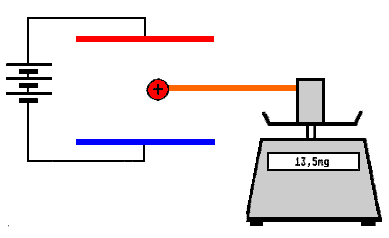
\includegraphics[width=0.5\textwidth]{img/efeldwaag_ladungenober_ver.png}
						\caption{Elektrische Feldstärke wiegen.}
						\label{img:efeldwaag_ladungenober_ver}
					\end{figure}
				
				\paragraph{Millikan-Versuch}
					
					Beim Millikonversuch werden leicht geladene Öltropfchen in einen Plattenkondesator gegeben. Wenn man die Spannung des Kondensators so einstellt, dass die Tröpfchen schweben, gilt
					\begin{equation}\label{millikan:f_g}
						F_G=F_{el}\Leftrightarrow m\cdot g = q\cdot \vec{E} = q\cdot\frac{U}{d}
					\end{equation}
					Da man $m$ aufgrund der kleinen Werte nicht direkt bestimmen kann, lässt man die Öltropfchen in dem ausgeschalteten Plattenkondensator sinken. aufgrund von Reibungskräften wird eine maximale Geschwindigkeit erreicht, mit der man dann durch die Formel $F_G=m\cdot g =F_R$ die Masse erhällt.\\
					Mit Gleichung \ref{millikan:f_g} kann man die Ladung der Öltropfchen bestimmen. Bei der Auswertung fällt auf, dass nur ganzzahlige Vielfache von $1.662\cdot 10^{-29}C$ auftreten. Das lässt darauf schließen, dass dies eine \textit{unteilbare} Elementarladung und damit die Ladung eines Elektrons sein muss.
					
				\paragraph{Elektronenstrahlröhre}
					Eine Elektronenstrahlröhre ist ein Gerät, in dem Elektronen erst beschleunigt und dann abgelenkt werden. Auf diese Weise ist es möglich zweidimensionale Bilder auf einen Schirm zu projezieren.
					\begin{figure}[H]
						\centering
						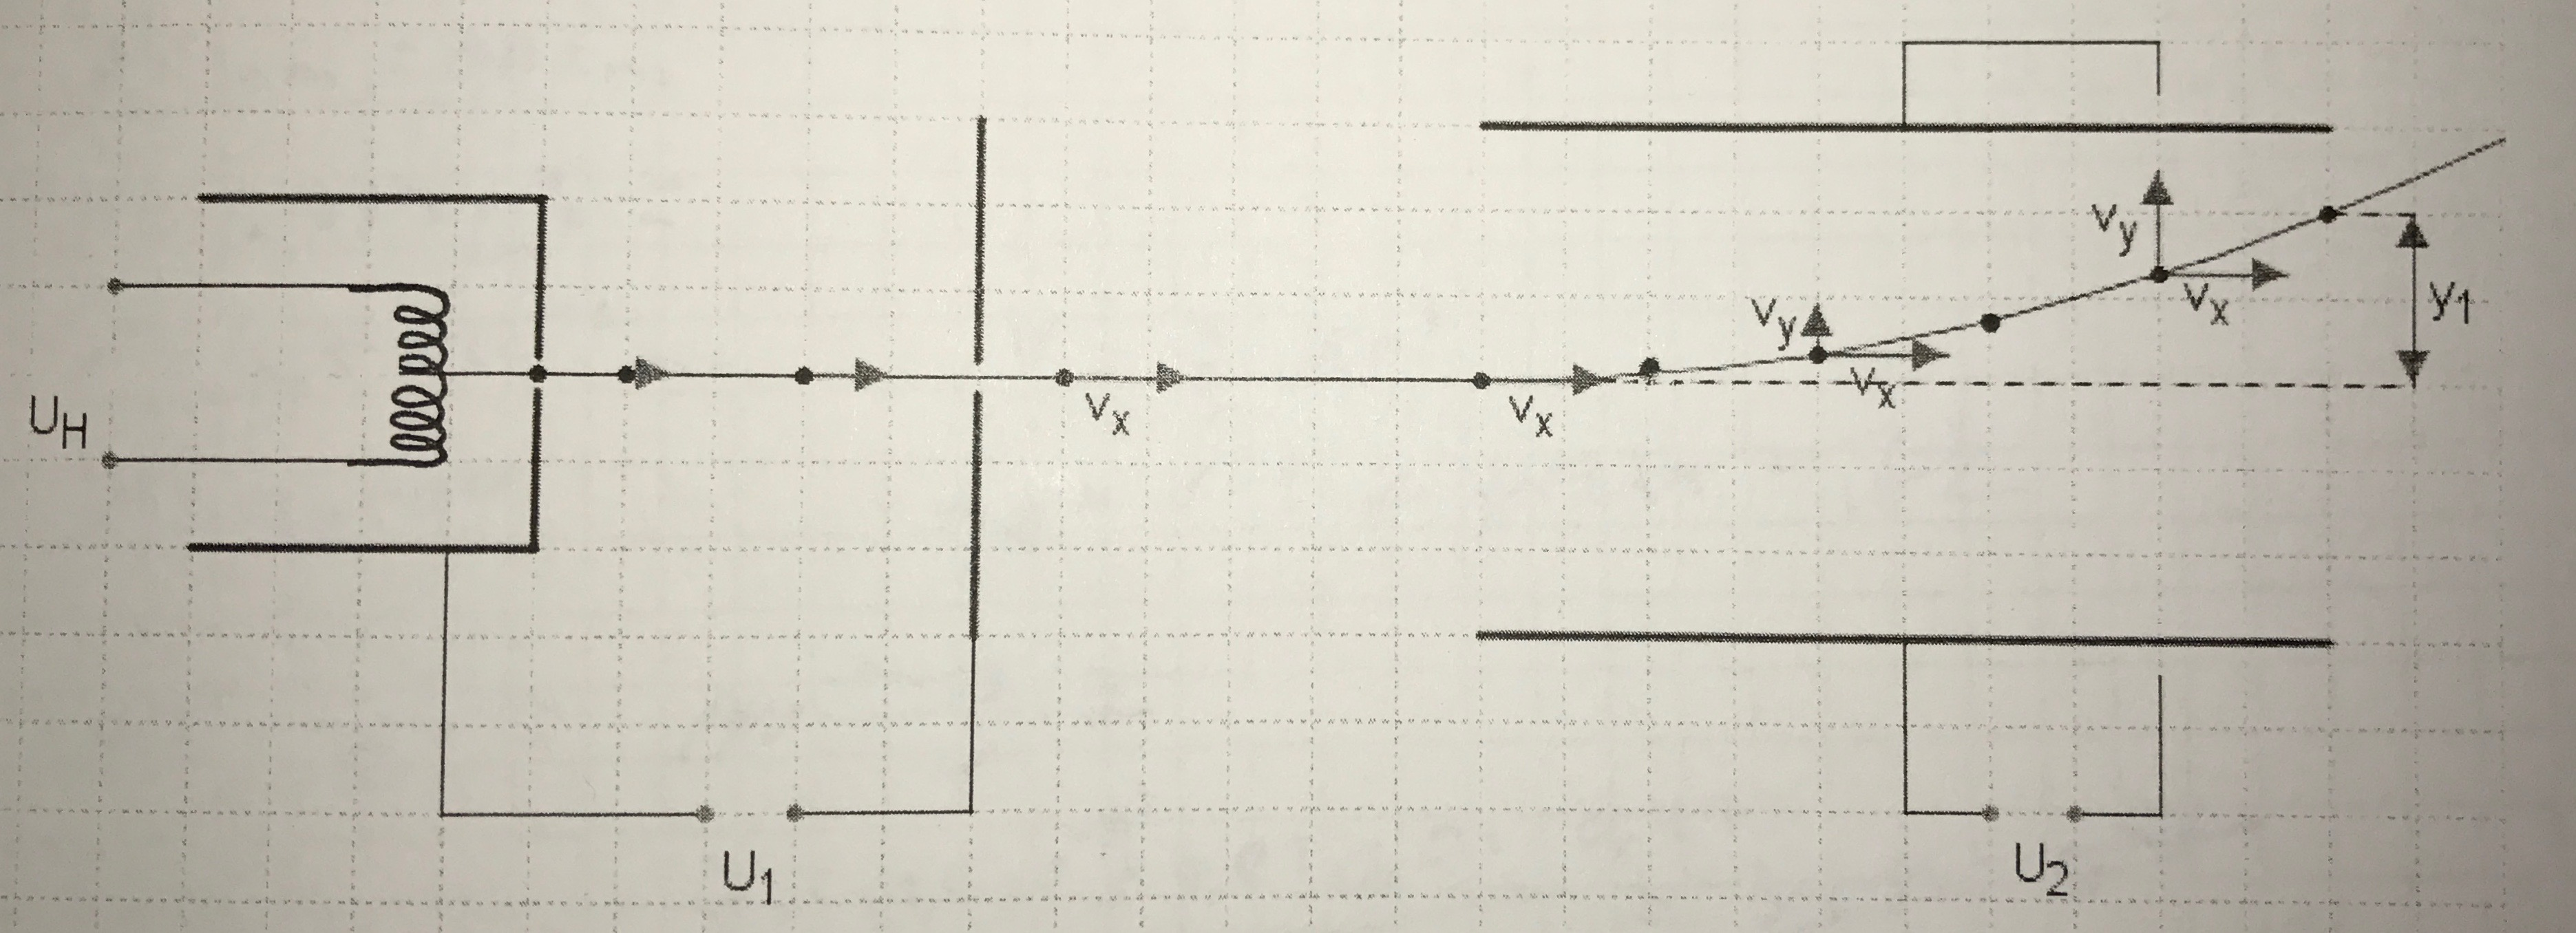
\includegraphics[width=0.8\textwidth]{img/elektronenstrahlroehre.jpg}
						\caption{Der Elektronenstrahlröhre}
						\label{img:elektronenstrahlroehre}
					\end{figure}
					\noindent Zuerst werden die Elektronen in dem ersten Plattenkondensator mit der Spannung $U_1$ beschleunigt. Dabei erhalten sich nach Gleichung  \ref{energie_kin_eq} und \ref{elektrisches_feld:beschleunigung_elektron} folgende Geschwindigkeit in x-Richtung:
					
					\begin{equation}
						\frac{1}{2}\cdot m_e \cdot v_x^2 = e \cdot U_1 \Leftrightarrow v_x = \sqrt{\frac{2\cdot e\cdot U_1}{m_e}}
					\end{equation}
					Die x-Geschwindigkeit ändert sich im zweiten Plattenkondensator mit dem Plattenabstand $d$ und der Länge $l$ nicht mehr, da hier nur eine Kraft in y-Richtung wirkt.\\
					Das Elektron braucht nach dem Bewegungsgesetzen der Mechanik folgende Zeit um den zweiten Plattenkondensator zu durchlaufen:
					
					\begin{equation}
						t=\frac{l}{v_x}\Leftrightarrow t=\frac{l}{\sqrt{\frac{2\cdot e\cdot U_1}{m_e}}}
					\end{equation}
					Setzt man  $\vec{E}=\frac{\vec{F_{el}}}{Q}$ mit $\vec{E}=\frac{U}{d}$ (Gleichung \ref{plattenkondensator:e}) gleich, erhällt man
					
					\begin{equation}
						\vec{F_{el}} = \frac{U_2}{d}\cdot e
					\end{equation}
					Mit Newtons Gleichung $F=m\cdot a$ kann man die Beschleunigung in y-Richtung im zweiten Plattenkondensator berechnen:
					
					\begin{equation}
						a = \frac{U_2\cdot e}{d\cdot m_e}
					\end{equation}
					Die Ablenkung $y_1$ im zweiten Kondensator ist dann:
					
					\begin{equation}
						y_1 = \frac{1}{2}\cdot a \cdot t^2 = \frac{1}{2}\cdot \frac{U_2\cdot e}{d\cdot m_e} \cdot \frac{l^2}{\frac{2\cdot e\cdot U_1}{m_e}}=\frac{U_2\cdot l^2}{4\cdot U_1\cdot d}
					\end{equation}
					
					Die Geschwindigkeit $v_y$ beträgt nach dem zweiten Kondensator:
					
					\begin{equation}
						v_y = a\cdot t = \frac{U_2\cdot e}{d\cdot m_e} \cdot \frac{l}{\sqrt{\frac{2\cdot e\cdot U_1}{m_e}}}
					\end{equation}
					
					
	
		\subsection{Magnetische Felder}
	\section{Quantenphysik des Lichtes}
	\section{Lichtelektrischer Effekt}
		\subsubsection{Röntgenspektren}
		\subsubsection{Compton Effect}
	\section{Quantenobjekte}

\end{document}
